\documentclass[12pt,a4paper]{article}
\usepackage{ctex}
\usepackage{amsmath,amscd,amsbsy,amssymb,latexsym,url,bm,amsthm}
\usepackage{epsfig,graphicx,subfigure}
\usepackage{enumitem,balance}
\usepackage{wrapfig}
\usepackage{mathrsfs,euscript}
\usepackage[usenames]{xcolor}
\usepackage{hyperref}
\usepackage[vlined,ruled,linesnumbered]{algorithm2e}
\hypersetup{colorlinks=true,linkcolor=black}
\usepackage[dvipsnames]{xcolor}
\usepackage{subcaption}
\usepackage{float}
\usepackage{graphicx}
\usepackage{graphicx}

\newtheorem{theorem}{Theorem}
\newtheorem{lemma}[theorem]{Lemma}
\newtheorem{proposition}[theorem]{Proposition}
\newtheorem{corollary}[theorem]{Corollary}
\newtheorem{exercise}{Exercise}
\newtheorem*{solution}{Solution}
\newtheorem{definition}{Definition}
\theoremstyle{definition}

\renewcommand{\thefootnote}{\fnsymbol{footnote}}

\newcommand{\postscript}[2]
 {\setlength{\epsfxsize}{#2\hsize}
  \centerline{\epsfbox{#1}}}

\renewcommand{\baselinestretch}{1.0}

\setlength{\oddsidemargin}{-0.365in}
\setlength{\evensidemargin}{-0.365in}
\setlength{\topmargin}{-0.3in}
\setlength{\headheight}{0in}
\setlength{\headsep}{0in}
\setlength{\textheight}{10.1in}
\setlength{\textwidth}{7in}
\makeatletter \renewenvironment{proof}[1][Proof] {\par\pushQED{\qed}\normalfont\topsep6\p@\@plus6\p@\relax\trivlist\item[\hskip\labelsep\bfseries#1\@addpunct{.}]\ignorespaces}{\popQED\endtrivlist\@endpefalse} \makeatother
\makeatletter
\renewenvironment{solution}[1][Solution] {\par\pushQED{\qed}\normalfont\topsep6\p@\@plus6\p@\relax\trivlist\item[\hskip\labelsep\bfseries#1\@addpunct{.}]\ignorespaces}{\popQED\endtrivlist\@endpefalse} \makeatother

\begin{document}
\noindent

%========================================================================
\noindent\framebox[\linewidth]{\shortstack[c]{
\Large{\textbf{Lab05-TM\&Complexity}}\vspace{1mm}\\
CS2312-Algorithm and complexity, Xiaofeng Gao, Spring 2026.}}
\begin{center}
\footnotesize{\color{red}$*$ Contact TA Steven Chen for any questions. Include both your .pdf and .tex files in the uploaded .rar or .zip file.}

% Please write down your name, student id and email.
\footnotesize{\color{blue}$*$ Name:HengtaoWu\quad Student ID:524031910038 \quad Email: Eternity\_w@sjtu.edu.cn}
\end{center}


\begin{enumerate}
    % -------------------------------
    % Question 1
    % -------------------------------
    \item {\color{purple}{(Turing Machine)}} 
    
    Given two sorted non-empty 3-bit binary integer arrays \(nums_1\) and \(nums_2\) in non-decreasing order, construct a 3-tape Deterministic Turing Machine that outputs the merged sorted array in non-decreasing order. The input tape is read-only.
    
    \textbf{Initial Configuration.}
    \[
        \begin{array}{|*{26}{c|}}
        \hline
        q_s \rightarrow & \triangleright & 0 & 0 & 1 & | & 0 & 1 & 0 & | & 0 & 1 & 1 & \# & 0 & 1 & 0 & | & 1 & 0 & 1 & | & 1 & 1 & 0 & \triangleleft \\
        \hline
        q_s \rightarrow & \triangleright & \multicolumn{24}{c|}{} \\
        \hline
        q_s \rightarrow & \triangleright & \multicolumn{24}{c|}{} \\
        \hline
        
        \end{array}
    \]
    

    \textbf{Alphabets. $\Gamma = \{0,1,\triangleright,\ \triangleleft,\ \vert,\ \#, \square\}$}

    \begin{itemize}
        \item \(\triangleright\) denotes the left-end marker,
        \item \(\triangleleft\) denotes the right-end marker,
        \item \(\#\) denotes the delimiter between arrays,
        \item \(\vert\) denotes the delimiter between integers in an array,
        \item \(\square\) denotes blank.
    \end{itemize}

    

    \begin{enumerate}
        \item Design an instruction set of the form:  
        \[
        \langle q_i,s^1_{j_1}, s^2_{j_2}, s^3_{j_3} \rangle \rightarrow \langle q_l,s^2_{k_2}, s^3_{k_3}, L/R/S, L/R/S, L/R/S \rangle.
        \]

        For example, suppose the machine is currently in state $q_s$, and all three tape heads are scanning the left-end marker $\triangleright$. We may move all three tape heads one cell to the right without changing the tape contents, while transitioning to state $q_1$. The corresponding instruction is:

        \[
        \langle q_s, \triangleright, \triangleright, \triangleright\rangle
        \rightarrow \langle q_1, \triangleright, \triangleright, R, R, R \rangle
        \]
        
        \item Briefly show the whole process from the initial to the final configuration, where the input arrays are $nums_1 = [1, 2, 3]$ and $nums_2 = [2, 5, 6]$, and the output array is $[1, 2, 2, 3, 5, 6]$. For example:
        \[
        (q_s, \underline{\triangleright} 001|010|011\#010|101|110 \triangleleft, \underline{\triangleright}, \underline{\triangleright}) \vdash (q_1, \triangleright \underline{0}01|010|011\#010|101|110 \triangleleft, \underline{\triangleright}, \underline{\triangleright}) 
        \]
        \[
        \vdash \cdots \vdash (q_h, \triangleright 001|010|011\#010|101|110 \underline{\triangleleft}, \cdots, \triangleright 001|010|010|011|101|110 \underline{\triangleleft})
        \]

        
    \end{enumerate}

    {\color{blue}{
        
    Note: You do not have to write out the non-transitioning tapes fully. For example, if only tape 1 changes state, you may write 
    \[
    (q_s, \underline{\triangleright} 001|010|011\#010|101|110 \triangleleft, \underline{\triangleright}, \underline{\triangleright}) \vdash (q_1, \triangleright \underline{0}01|010|011\#010|101|110 \triangleleft, \dots, \dots)
    \]
    If the same instruction executes repeatedly, you may skip the intermediate transitions. For example, if your instruction consecutively shifts the first tape pointer to the right, you may skip from 
    \[(q_s, \underline{\triangleright} 001|010|011\#010|101|110 \triangleleft, \underline{\triangleright}, \underline{\triangleright}) \vdash^* (q_1, \triangleright 001|010|011\underline{\#}010|101|110 \triangleleft, \underline{\triangleright}, \underline{\triangleright})
    \]
    
    }}

    \begin{solution}
        \begin{enumerate}
            \item We use tape 1 as the read-only input tape, tape 2 as a working tape storing \(nums_1\), and tape 3 as the output tape. The machine first copies \(nums_1\) from tape 1 to tape 2, then compares the current 3-bit integer on tape 1 with the current 3-bit integer on tape 2. Tape 1 stores the current pointer of \(nums_2\), tape 2 stores the current pointer of \(nums_1\), and tape 3 stores the merged output.

            Let \[ B=\{0,1\}, \qquad D_1=\{\vert,\#\}, \qquad D_2=\{\vert,\triangleright\}. \] Here \(D_1\) is the set of left delimiters on tape 1 when the head moves back to the beginning of a number, and \(D_2\) is the corresponding set on tape 2.

            \medskip \noindent\textbf{Start state.} \[ \langle q_s,\triangleright,\triangleright,\triangleright\rangle \to \langle q_1,\triangleright,\triangleright,R,R,R\rangle . \]

            \medskip 
            \noindent\textbf{State \(q_1\): copy \(nums_1\) from tape 1 to tape 2.} 
            For \(a\in\{0,1,\vert\}\), \[ \langle q_1,a,\square,\square\rangle \to \langle q_1,a,\square,R,R,S\rangle . \]

            When the delimiter \(\#\) is met, the first array has been copied to tape 2. We write the right-end marker of tape 2 and move tape 1 to the beginning of \(nums_2\). \[ \langle q_1,\#, \square,\square\rangle \to \langle q_2,\triangleleft,\square,R,L,S\rangle . \]

            \medskip \noindent\textbf{State \(q_2\): move the head of tape 2 back to the beginning.} For \(b\in\{0,1,\vert\}\) and \(a\in\{0,1\}\), \[ \langle q_2,a,b,\square\rangle \to \langle q_2,b,\square,S,L,S\rangle . \] When the left-end marker on tape 2 is reached, move tape 2 one cell to the right and enter the compare state. \[ \langle q_2,a,\triangleright,\square\rangle \to \langle q_3,\triangleright,\square,S,R,S\rangle . \]


            \medskip \noindent\textbf{State \(q_3\): compare the current 3-bit integers.} If the current bits are equal, copy this bit to tape 3 and move all three heads to the right. For \(x\in B\), \[ \langle q_3,x,x,\square\rangle \to \langle q_3,x,x,R,R,R\rangle . \] If tape 2 has the smaller bit, namely tape 1 reads \(1\) and tape 2 reads \(0\), copy the \(0\) to tape 3 and enter \(q_4\), where the rest of the integer on tape 2 will be copied. \[ \langle q_3,1,0,\square\rangle \to \langle q_4,0,0,L,R,R\rangle . \]

            If tape 1 has the smaller bit, namely tape 1 reads \(0\) and tape 2 reads \(1\), copy the \(0\) to tape 3 and enter \(q_5\), where the rest of the integer on tape 1 will be copied. \[ \langle q_3,0,1,\square\rangle \to \langle q_5,1,0,R,L,R\rangle . \] If both heads reach \(\vert\), the two 3-bit integers are equal. One copy has already been written to tape 3. We move tape 1 back to the beginning of this integer, keep tape 2 at the delimiter, and use \(q_4\) to finish this adjustment. Then tape 2 moves to its next integer, while tape 1 keeps this equal integer for the next comparison. This can be simplified to state \textbf{State \(q_4\)}. \[ \langle q_3,\vert,\vert,\square\rangle \to \langle q_4,\vert,\vert,L,S,S\rangle . \]

            If tape 2 reaches \(\triangleleft\), then all elements of \(nums_1\) have been used. The machine copies the remaining elements of \(nums_2\) from tape 1 to tape 3. \[ \langle q_3,a,\triangleleft,\square\rangle \to \langle q_{\mathrm{rem1}},\triangleleft,\square,S,S,S\rangle , \qquad a\in\{0,1,\vert\}. \] If tape 1 reaches \(\triangleleft\), then all elements of \(nums_2\) have been used. The machine copies the remaining elements of \(nums_1\) from tape 2 to tape 3. \[ \langle q_3,\triangleleft,b,\square\rangle \to \langle q_{\mathrm{rem2}},b,\square,S,S,S\rangle , \qquad b\in\{0,1,\vert\}. \]

            \medskip
            \noindent\textbf{State \(q_4\): copy the current integer on tape 2.} 
            State \(q_4\) is used when the current integer on tape 2 should be output. At the same time, the head of tape 1 moves back to the beginning of its current integer. 
            
            For \(a,b\in B\):
            \[
            \langle q_4,a,b,\square\rangle \to \langle q_4,b,b,L,R,R\rangle .
            \]
            
            If tape 1 has already reached the delimiter on the left of its current integer, but tape 2 still reads a bit, then tape 1 stays and tape 2 continues copying. For \(d\in D_1\) and \(b\in B\):
            \[
            \langle q_4,d,b,\square\rangle \to \langle q_4,b,b,S,R,R\rangle .
            \]
            
            If tape 2 has reached the delimiter but tape 1 has not moved back enough, then only tape 1 moves left. For \(a\in B\):
            \[
            \langle q_4,a,|,\square\rangle \to \langle q_4,|,|,L,S,S\rangle .
            \]
            
            % 新增处理终止符
            If tape 2 has reached the right-end marker:
            \[
            \langle q_4,a,\triangleleft,\square\rangle \to \langle q_3,a,\triangleleft,R,S,S\rangle .
            \]
            
            When tape 1 has reached the left delimiter and tape 2 has reached the right delimiter of the copied integer (| or $\triangleleft$), the current integer on tape 2 has been fully copied. We write a delimiter on tape 3 and move both input pointers to the next integers. For \(d\in D_1\):
            \[
            \langle q_4,d,|,\square\rangle \to \langle q_3,|,|,R,R,R\rangle ,\quad
            \langle q_4,d,|,|\rangle \to \langle q_3,|,|,R,R,R\rangle .
            \]
            
            \medskip
            \noindent\textbf{State \(q_5\): copy the current integer on tape 1.} 
            State \(q_5\) is symmetric to \(q_4\). It is used when the current integer on tape 1 should be output. At the same time, the head of tape 2 moves back to the beginning of its current integer. 
            
            For \(a,b\in B\):
            \[
            \langle q_5,a,b,\square\rangle \to \langle q_5,b,a,R,L,R\rangle .
            \]
            
            If tape 2 has already reached the left delimiter of its current integer, but tape 1 still reads a bit, tape 2 stays and tape 1 continues copying. For \(a\in B\) and \(d\in D_2\):
            \[
            \langle q_5,a,d,\square\rangle \to \langle q_5,d,a,R,S,R\rangle .
            \]
            
            If tape 1 has reached the delimiter but tape 2 has not moved back enough, then only tape 2 moves left. For \(b\in B\):
            \[
            \langle q_5,|,b,\square\rangle \to \langle q_5,b,|,S,L,S\rangle .
            \]
            
            % 新增处理终止符
            If tape 1 has reached the right-end marker:
            \[
            \langle q_5,\triangleleft,b,\square\rangle \to \langle q_3,\triangleleft,b,R,S,S\rangle .
            \]
            
            When tape 1 has reached the right delimiter of the copied integer and tape 2 has reached the left delimiter of its current integer (| or $\triangleleft$ ), the current integer on tape 1 has been fully copied. We write a delimiter on tape 3 and move both input pointers to the next integers. For \(d\in D_2\):
            
            \[
            \langle q_5,|,d,\square\rangle \to \langle q_3,d,|,R,R,R\rangle ,\quad
            \langle q_5,|,d,|\rangle \to \langle q_3,d,|,R,R,R\rangle .
            \]
            
            
            \medskip \noindent\textbf{Copy the remaining elements.} If all elements on tape 2 have been consumed, state \(q_{\mathrm{rem1}}\) copies the remaining symbols on tape 1 to tape 3: \[ \langle q_{\mathrm{rem1}},a,b,\square\rangle \to \langle q_{\mathrm{rem1}},b,a,R,S,R\rangle , \qquad a\in\{0,1,\vert\}. \] When the right-end marker is reached, the machine halts: \[ \langle q_{\mathrm{rem1}},\triangleleft,b,\square\rangle \to \langle q_h,b,\triangleleft,S,S,S\rangle . \] 
            
            Similarly, if all elements on tape 1 have been consumed, state \(q_{\mathrm{rem2}}\) copies the remaining symbols on tape 2 to tape 3: \[ \langle q_{\mathrm{rem2}},a,b,\square\rangle \to \langle q_{\mathrm{rem2}},b,b,S,R,R\rangle , \qquad b\in\{0,1,\vert\}. \] When the right-end marker on tape 2 is reached, the machine halts: \[ \langle q_{\mathrm{rem2}},a,\triangleleft,\square\rangle \to \langle q_h,\triangleleft,\triangleleft,S,S,S\rangle . \]
            
            
            
            \item Computation process example.

            Let \(nums_1 = [001, 010, 011]\) and \(nums_2 = [010, 101, 110]\).

            \medskip

            \noindent\textbf{Start and copy phase:}
        \[
        (q_s, \underline{\triangleright}001|010|011\#010|101|110\triangleleft, \underline{\triangleright}, \underline{\triangleright})
        \vdash
        (q_1, \triangleright \underline{0}01|010|011\#010|101|110\triangleleft, \dots, \dots)
        \]
        \[\
        \vdash^* 
        (q_1, \triangleright 001|010|011\underline{\#}010|101|110\triangleleft, \dots, \dots)
        \vdash
        (q_2, \triangleright 001|010|011\triangleleft, \underline{0}10|101|110, \underline{\triangleright})
        \]
        
        \medskip
        \noindent\textbf{Go back:}
        \[
        (q_2, \triangleright 001|010|011\triangleleft, \underline{0}10|101|110, \underline{\triangleright})
        \vdash^* 
        (q_3, \underline{0}01|010|011\triangleleft, \underline{0}10|101|110, \underline{\triangleright})
        \]
        
        \medskip
        \noindent\textbf{Compare and merge (simplified using your rules):}
        
        \[
        (q_3, \underline{0}01|010|011\triangleleft, \underline{0}10|101|110, \underline{\triangleright})
        \vdash
        (q_3, 0\underline{0}1|010|011\triangleleft, 0\underline{1}0|101|110, 0\underline{0}\square\dots)
        \vdash^* 
        (q_4, \dots)
        \]
        
        \[
        \vdash^* 
        (q_3, \triangleright 001|010|011\#0\underline{1}0|101|110\triangleleft, \dots, \triangleright 001|010|010|011\dots)
        \]
        
        \[
        \vdash^* 
        (q_3, \dots, \dots, \dots)
        \vdash^* 
        (q_h, \triangleright 001|010|010|011|101|110 \triangleleft, \dots, \triangleright 001|010|010|011|101|110 \triangleleft)
        \]
        
        \medskip
        Here we use:
        \begin{itemize}
            \item \(\vdash^*\) to indicate repeated application of the same instruction (e.g., moving right through bits of a number).
            \item Ellipsis (\(\dots\)) to indicate tape contents that do not change or are not relevant at this step.
            \item The states \(q_4, q_5\) handle fully copying the smaller number to the output tape and adjusting the head positions.
        \end{itemize}
                    
        \end{enumerate}
    \end{solution}
    
    
    % -------------------------------
    % Question 2
    % -------------------------------
    \item {\color{purple}(Reduction via Gadgets)} 
    
    The Steiner Tree (ST) problem: Given an undirected, unweighted, connected graph $G = (V, E)$, and a subset $S$ of the nodes of $G$ (the shaded nodes), plus a non-negative integer $k$, is there a subset $E'$ of edges of $G$ that connects all of the shaded nodes, where $|E'| \leq k$?

    \begin{enumerate}
        \item Show that the ST problem is in NP.
        \item Describe an efficient reduction from the 3-SAT to the ST problem.
        
        \item Prove the correctness of your reduction by showing that instance $\Phi$ is a Yes-instance of 3-SAT if and only if instance $I = (G, S, k)$ is a Yes-instance of ST.
    \end{enumerate}


\begin{solution}
    \begin{enumerate}
        \item 
        We show that the Steiner Tree problem is in NP.

        A certificate for an instance \((G,S,k)\) is a subset of edges
        \(E'\subseteq E\). Given \(E'\), we can check in polynomial time that
        \[
        |E'|\leq k.
        \]
        Then we consider the subgraph \(G'=(V,E')\), and run a graph search
        algorithm, such as BFS or DFS, from any node in \(S\). We accept if and
        only if all nodes in \(S\) are reached. This verifies that all shaded
        nodes are connected by \(E'\).

        Since the size of the certificate is polynomial in the input size and
        the verification can be done in polynomial time, the Steiner Tree
        problem is in NP.

        \item 
        We describe a polynomial-time reduction from 3-SAT to the Steiner Tree
        problem.

        Let
        \[
        \Phi=C_1\land C_2\land\cdots\land C_m
        \]
        be a 3-SAT formula over variables
        \[
        x_1,x_2,\dots,x_n.
        \]
        Each clause \(C_j\) has exactly three literals. We construct an
        undirected, unweighted graph \(G=(V,E)\), a set \(S\) of shaded nodes,
        and an integer \(k\).

        First, we construct the variable gadgets. We create nodes
        \[
        v_0,v_1,\dots,v_n.
        \]
        For each variable \(x_i\), we create two literal nodes \(x_i\) and
        \(\neg x_i\). Then we add the following four edges:
        \[
        (v_{i-1},x_i),\quad (x_i,v_i),
        \]
        and
        \[
        (v_{i-1},\neg x_i),\quad (\neg x_i,v_i).
        \]
        Thus, between \(v_{i-1}\) and \(v_i\), there are two paths of length
        two. Choosing the path through \(x_i\) will represent setting
        \(x_i=\mathrm{True}\), while choosing the path through \(\neg x_i\)
        will represent setting \(x_i=\mathrm{False}\).

        Next, we construct the clause gadgets. For each clause \(C_j\), create
        one node \(c_j\). This node will be a shaded node. If
        \[
        C_j=(\ell_{j1}\lor \ell_{j2}\lor \ell_{j3}),
        \]
        where each \(\ell_{jt}\) is a literal, then we add the three edges
        \[
        (c_j,\ell_{j1}),\quad (c_j,\ell_{j2}),\quad (c_j,\ell_{j3}).
        \]
        In other words, the clause node \(c_j\) is adjacent exactly to the
        three literal nodes that appear in \(C_j\).

        The set of shaded nodes is
        \[
        S=\{v_0,v_n,c_1,c_2,\dots,c_m\}.
        \]
        Finally, we set
        \[
        k=2n+m.
        \]

        This construction is clearly polynomial in the size of \(\Phi\), since
        it creates \(O(n+m)\) nodes and edges.


        \begin{figure}[htbp]
        \centering
        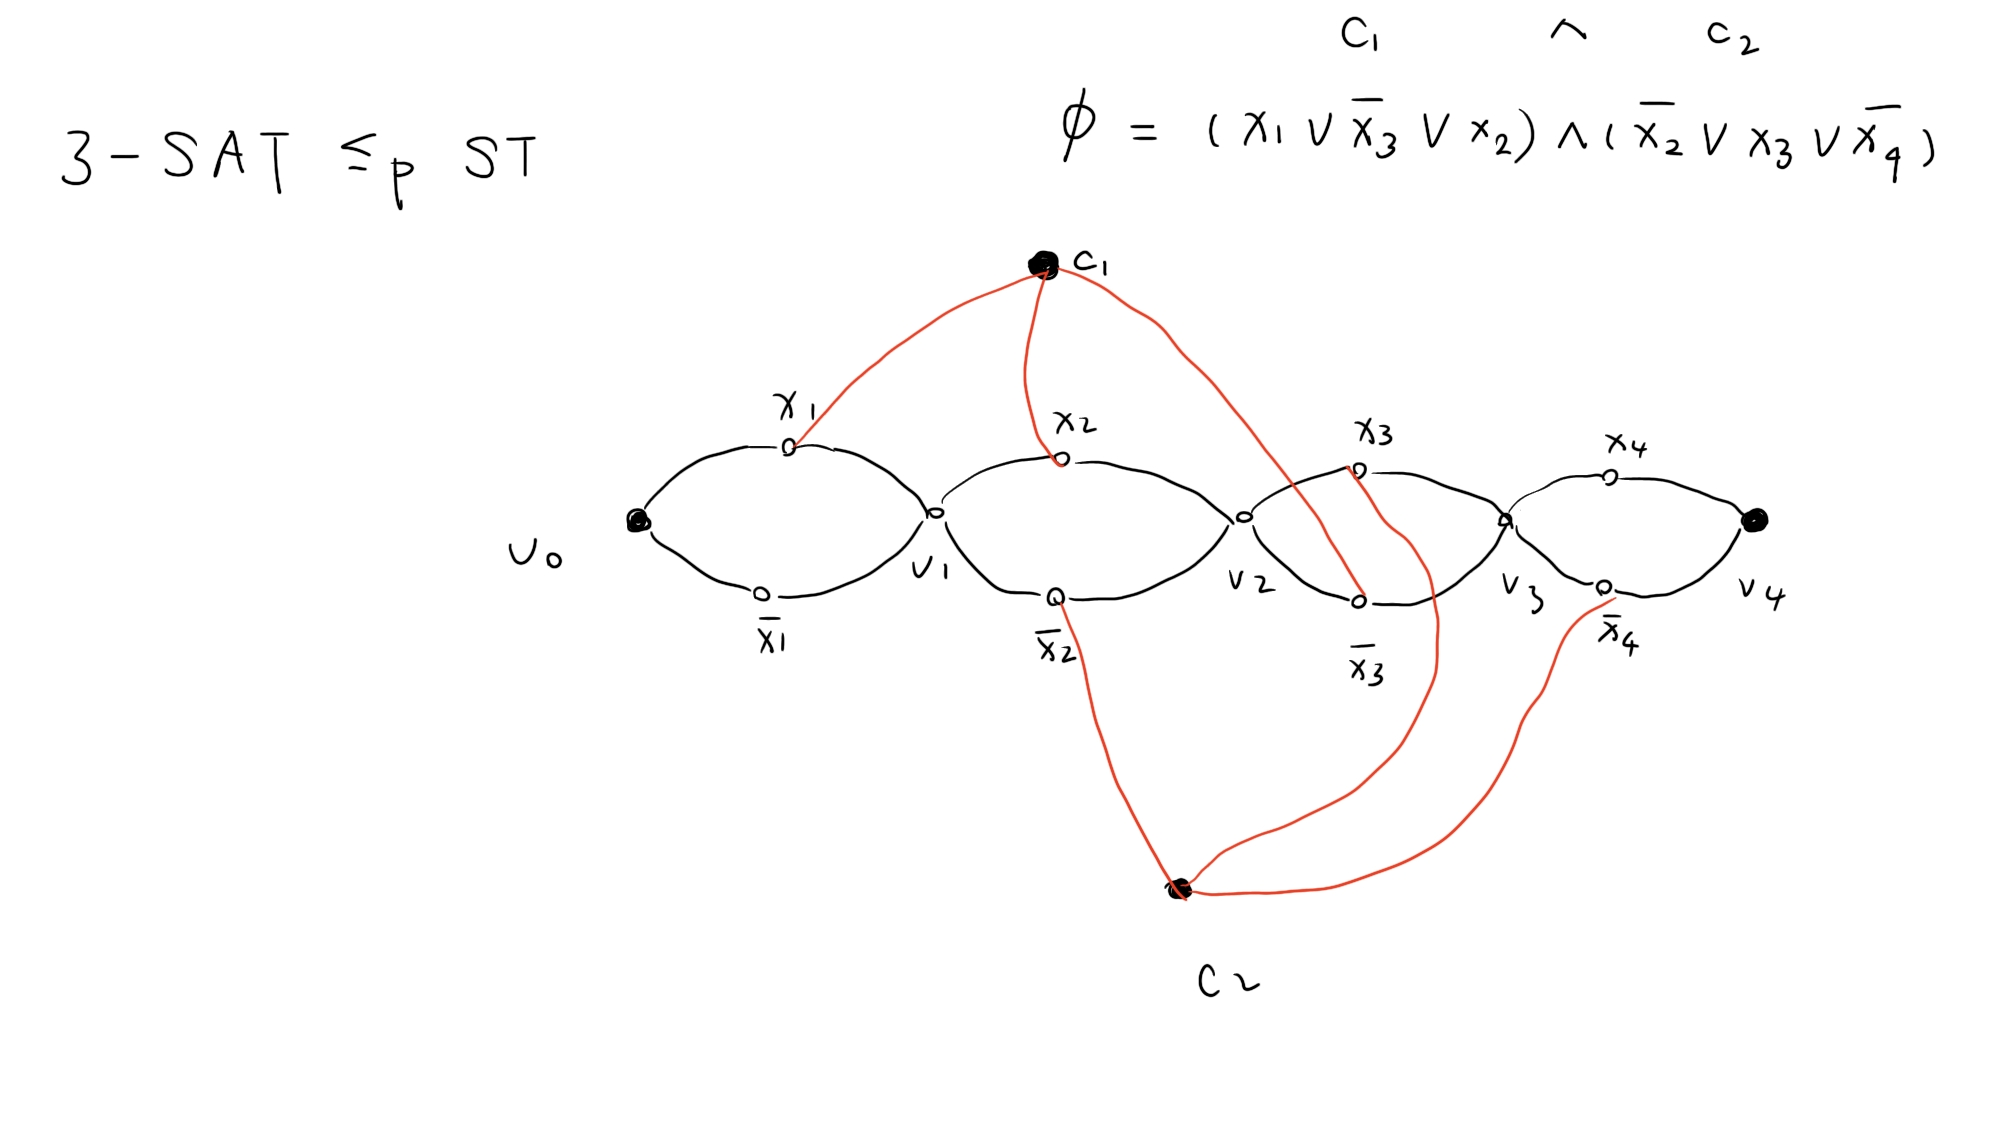
\includegraphics[width=0.8\textwidth]{1.jpg}
        \caption{Example for the construction.}
        \label{fig:example}
        \end{figure}


        \item
        We prove the correctness of the reduction. We show that
        \[
        \Phi \text{ is satisfiable}
        \iff
        (G,S,k) \text{ is a Yes-instance of ST}.
        \]

        \medskip

        \noindent\textbf{(\(\Rightarrow\))} Suppose \(\Phi\) is satisfiable.
        Let \(\alpha\) be a satisfying assignment.

        We construct a set of edges \(E'\) as follows. For each variable
        \(x_i\), if \(\alpha(x_i)=\mathrm{True}\), we include the two edges
        \[
        (v_{i-1},x_i),\quad (x_i,v_i).
        \]
        If \(\alpha(x_i)=\mathrm{False}\), we include the two edges
        \[
        (v_{i-1},\neg x_i),\quad (\neg x_i,v_i).
        \]
        Therefore, these selected edges form a path from \(v_0\) to \(v_n\),
        and the number of such edges is \(2n\).

        Now consider any clause \(C_j\). Since \(\alpha\) satisfies \(\Phi\),
        the clause \(C_j\) contains at least one true literal. Let
        \(\ell\) be such a true literal in \(C_j\). By our construction,
        \(c_j\) is adjacent to the literal node \(\ell\). Also, since
        \(\ell\) is true under the chosen assignment, the literal node
        \(\ell\) lies on the selected path from \(v_0\) to \(v_n\). Therefore,
        we add the edge
        \[
        (c_j,\ell)
        \]
        to \(E'\). We do this for every clause \(C_j\), adding exactly one
        edge per clause, for a total of \(m\) additional edges.

        Hence
        \[
        |E'|=2n+m=k.
        \]
        Moreover, the edges in \(E'\) connect \(v_0\), \(v_n\), and every
        clause node \(c_j\). Thus all shaded nodes in \(S\) are connected.
        Therefore, \((G,S,k)\) is a Yes-instance of ST.

        \medskip

        \noindent\textbf{(\(\Leftarrow\))} Suppose \((G,S,k)\) is a
        Yes-instance of ST. Then there exists a set of edges \(E'\subseteq E\)
        such that \(|E'|\leq k=2n+m\), and all shaded nodes in
        \[
        S=\{v_0,v_n,c_1,c_2,\dots,c_m\}
        \]
        are connected by \(E'\).

        Since \(v_0\) and \(v_n\) are shaded nodes, they must be connected in
        the subgraph induced by \(E'\). In the constructed graph, any path from
        \(v_0\) to \(v_n\) must pass through each variable gadget from
        \(v_{i-1}\) to \(v_i\). For each \(i\), the only ways to go from
        \(v_{i-1}\) to \(v_i\) are through \(x_i\) or through \(\neg x_i\),
        and each such choice uses two edges. Thus, connecting \(v_0\) to
        \(v_n\) requires at least \(2n\) edges.

        Also, each clause node \(c_j\) is shaded, so it must be connected to
        the rest of the tree. Since \(c_j\) is not on the main variable path,
        connecting it requires at least one additional edge. Since there are
        \(m\) clause nodes, this requires at least \(m\) additional edges.

        Therefore, any feasible Steiner tree must use at least
        \[
        2n+m
        \]
        edges. But \(|E'|\leq k=2n+m\), so it must use exactly \(2n+m\) edges.
        This means that the tree has no extra edges. In particular, it chooses
        exactly one of the two paths in each variable gadget, and each clause
        node \(c_j\) is connected by exactly one edge to a literal node on the
        chosen variable path.

        We now define a truth assignment \(\alpha\). For each variable \(x_i\),
        if the selected path between \(v_{i-1}\) and \(v_i\) goes through
        \(x_i\), set
        \[
        \alpha(x_i)=\mathrm{True}.
        \]
        If it goes through \(\neg x_i\), set
        \[
        \alpha(x_i)=\mathrm{False}.
        \]

        Consider any clause \(C_j\). Since \(c_j\) is connected to the Steiner
        tree using exactly one edge, it is connected to one of the literal
        nodes appearing in \(C_j\). This literal node lies on the selected
        variable path, so it is true under the assignment \(\alpha\). Therefore,
        \(C_j\) has at least one true literal.

        Since this holds for every clause \(C_j\), the formula \(\Phi\) is
        satisfied by \(\alpha\). Hence \(\Phi\) is a Yes-instance of 3-SAT.

        Therefore,
        \[
        \Phi \text{ is satisfiable}
        \iff
        (G,S,k) \text{ is a Yes-instance of ST}.
        \]
        This completes the reduction from 3-SAT to ST.
    \end{enumerate}
\end{solution}



    % -------------------------------
    % Question 3
    % -------------------------------
    \newpage
    \item {\color{purple}{(NP-Complete)}} 
    
    A recruitment agency wishes to offer $n$ possible jobs. There are $k$ job seekers interested in getting a job and each is interested in some subset of the $n$ possible jobs. To manage costs, the agency has a bound $b$ on the number of jobs it is willing to offer. Is there a way to choose $b$ jobs out of the $n$ possibilities so that every job seeker can get a job that interests them? Formally, an instance of the Job Scheduling (JS) problem consists of
    
    \begin{itemize}
        \item a set $C$ of $n$ possible courses, numbered $1$ through $n$, 
        
        \item subsets $S_1, S_2, \dots, S_k \text{ of } \{1, 2, \dots, n\}$ (the jobs of interest to each of the job seekers), 
        
        \item and a bound $b$ (the maximum number of jobs actually offered).
    \end{itemize}

    The JS problem is to determine whether there is a subset $B$ of $\{1, 2, \dots, n\}$, where the size of $B \leq b$, such that $B \cap S_i$ is not empty for all $i, 1 \leq i \leq k$.

    \begin{enumerate}
        \item Describe an efficient reduction from the Vertex Cover problem to the JS problem.
        
        \item Show that your reduction runs in polynomial time.
        
        \item Show that the JS problem is NP-complete.
    \end{enumerate}


    \begin{solution}
        
    \begin{enumerate}
    \item Reduction construction:

    Given a Vertex Cover (VC) instance with graph \(G=(V,E)\) and bound \(k\), we construct a Job Scheduling (JS) instance as follows:
    \begin{itemize}
        \item Each vertex \(u \in V\) becomes a job in JS.
        \item Each edge \(e = \{u,v\} \in E\) becomes a job seeker, whose set of interesting jobs is exactly \(\{u,v\}\).
        \item Set the job bound \(b = k\), same as the VC bound.
    \end{itemize}

    \item Polynomial time:

    The construction is polynomial because:
    \begin{itemize}
        \item There is one job per vertex (\(|V|\) jobs).
        \item One job seeker per edge (\(|E|\) job seekers), each with at most two jobs.
        \item The bound \(b=k\) is directly taken from the VC instance.
    \end{itemize}
    Therefore the JS instance can be created in time polynomial in the size of the VC instance.

    \item Correctness:

    \textbf{(VC yes $\Rightarrow$ JS yes):} If the VC instance has a vertex cover of size \(\le k\), select the corresponding jobs in JS. Every edge \(e = \{u,v\}\) in VC is covered by at least one vertex in the cover, so the corresponding job seeker has at least one job in the selection. Hence all job seekers are satisfied and the job selection size \(\le b\).

    \textbf{(JS yes $\Rightarrow$ VC yes):} If there exists a subset of jobs \(B\) with \(|B| \le b\) satisfying all job seekers, then selecting the corresponding vertices in VC covers every edge (because each edge corresponds to a job seeker, who is satisfied only if at least one of its two jobs is in \(B\)). Thus, there exists a vertex cover of size \(\le k\).

    Since JS is in NP (a job selection can be verified in polynomial time), and VC \(\le_p\) JS, the JS problem is NP-complete.
\end{enumerate}

    \end{solution}
    
    
\end{enumerate}
%========================================================================
\end{document}
